
\documentclass{exam}

\usepackage{units} 
\usepackage{graphicx}
\usepackage[fleqn]{amsmath}
\usepackage{cancel}
\usepackage{float}
\usepackage{mdwlist}
\usepackage{booktabs}
\usepackage{cancel}
\usepackage{polynom}
\usepackage{caption}
\usepackage{fullpage}
\usepackage{xfrac}
\usepackage{enumerate}

\newcommand{\degree}{\ensuremath{^\circ}} 
\everymath{\displaystyle}

% \begin{figure}[H]
%   \centering
%   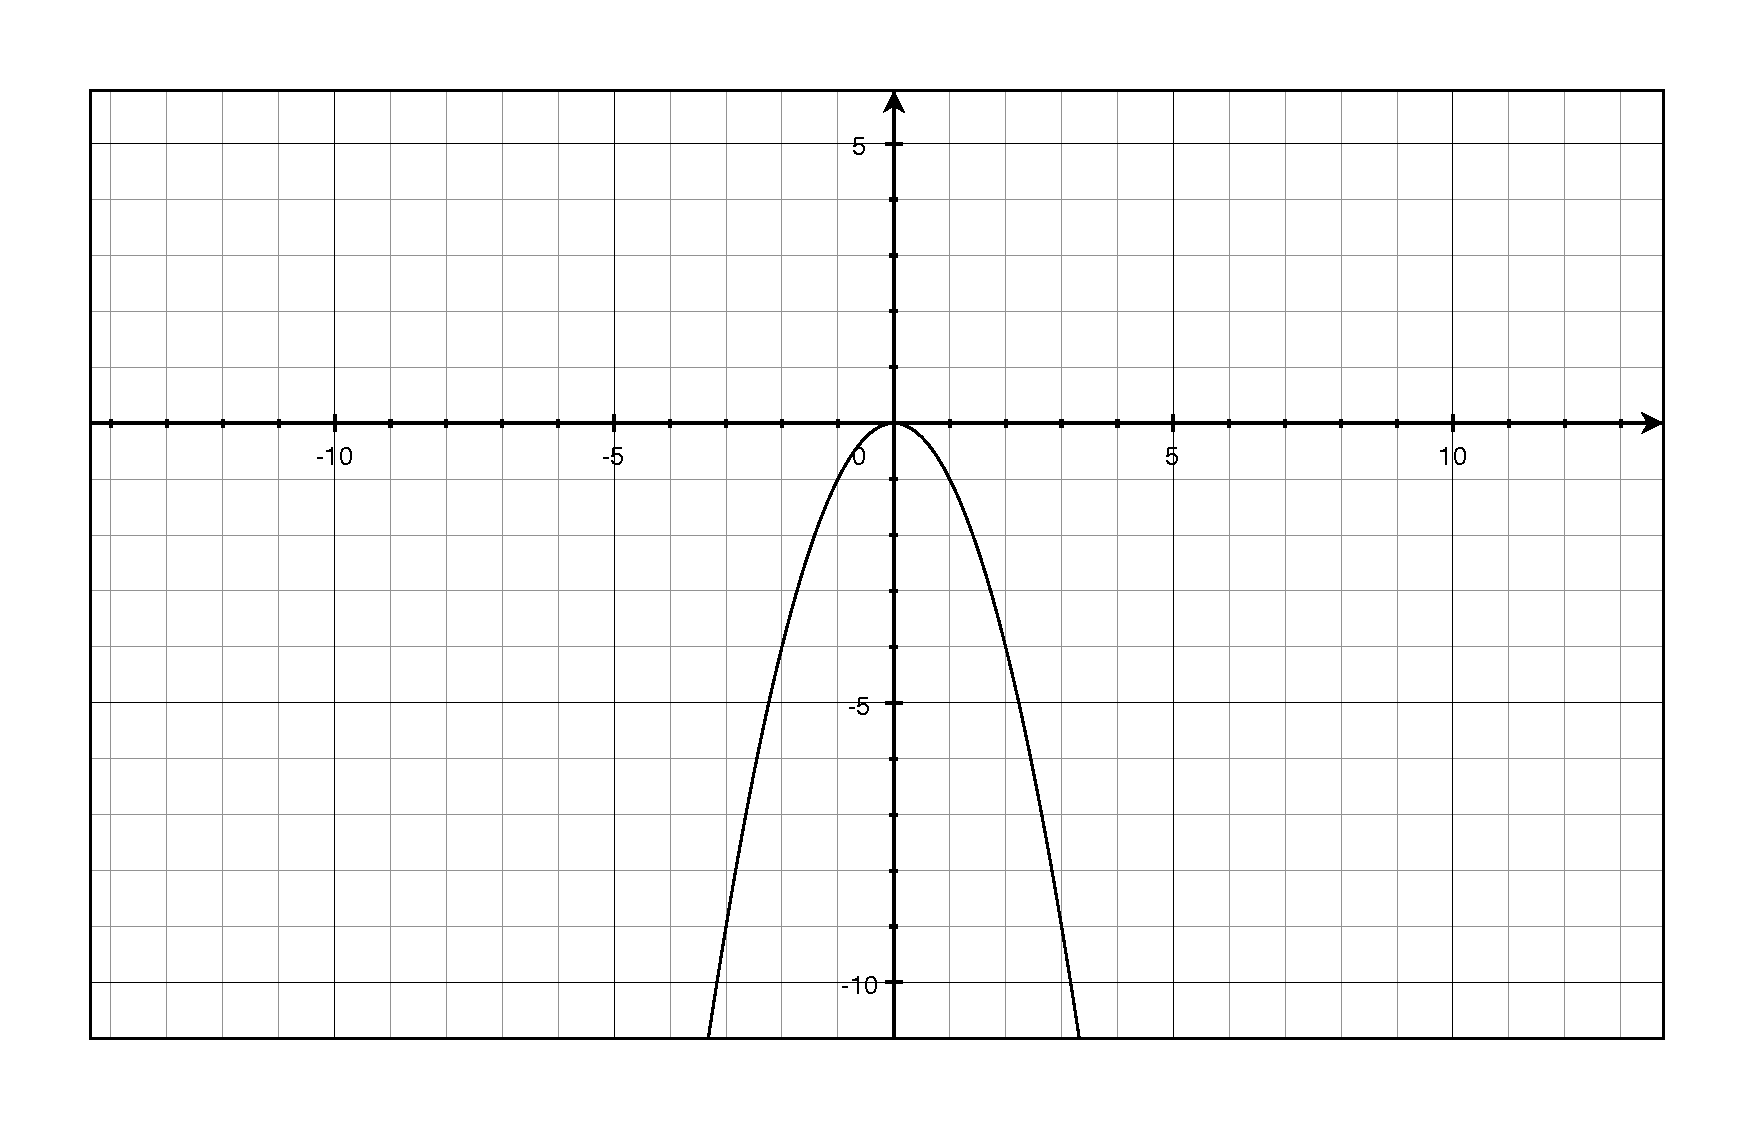
\includegraphics[scale=0.9]{problem7.eps}
%   \caption*{Problem 7}
% \end{figure}

% \begin{tabular}{cc}
%   \toprule
%   period & amplitude \\
%   \midrule
%   value one & value two
%   \bottomrule
% \end{tabular}

\printanswers

\ifprintanswers 
  \usepackage{2in1, lscape} 
\fi

\date{June 12, 2013}
\author{}
\title{Math 141 \\ Homework 14}

\begin{document}

  \maketitle

  \section{Homework}

  Section 4.2: 1-32, 37-46, 49-54, 58-81

 \section{Extra Credit}
  Section 4.2: 75-76

  \ifprintanswers
    \begin{description}
      \item[75]
        \begin{enumerate}[a]

          \item 
            \begin{align*}
              \log_{10} x      & > 0 \\
              10^{\log_{10} x} & > 10^0 \\
              x                & > 1 \\
            \end{align*}

            \fbox{$(1, \infty)$}

          \item 
            \begin{align*}
              y        &= \log_2 (\log_{10} x) \\
              2^y      &= \log_{10} x \\
              10^{2^y} &= x \\
            \end{align*}

            The inverse function is: \fbox{$f^{-1}(x) = 10^{2^x}$}

            % check:
            % \begin{align*}
            %   f^{-1}(f(x)) &= 10^{ 2^{ \log_2( \log_{10} x ) } } \\
            %                &= 10^{\log_{10} x} \\
            %                &= x \\
            %   \\
            %   f(f^{-1}(x)) &= \log_2 (\log_{10} 10^{2^x}) \\
            %                &= \log_2 2^x \\
            %                &= x \\
            % \end{align*}

          \item 
            \begin{align*}
              \ln(\ln x)     & > 0 \\
              e^{\ln(\ln x)} & > e^0 \\
              \ln x          & > 1 \\
              e^{\ln x}      & > e^1 \\
              x              & > e \\
            \end{align*}

            \fbox{$(e, \infty)$}

          \item 
            \begin{align*}
              y        &= \ln(\ln(\ln x)) \\
              e^y      &= \ln(\ln x) \\
              e^{e^y}      &= \ln x \\
              e^{e^{e^y}}      &= x \\
            \end{align*}

            The inverse function is: \fbox{$f^{-1}(x) = e^{e^{e^x}}$}
        \end{enumerate}
    \end{description}
  \fi

\begin{enumerate}
  \item 
    Remember that a definition of $e$ is:
    \[
      e \approx \left( 1 + \frac{1}{n} \right)^n
    \]
    where the approximation gets better as $n$ gets bigger.

    An interesting fact about $e^x$ is that $e^x \approx 1 + x$ when $x$ is a small number.  Explain why.

  \item 
    When calculating the base 10 logarithm table, Napier noticed that for small $x$:
    \[
      \log_{10} x \approx 1 + 2.3026x
    \]

    Where does the number 2.3026 come from and why does $\log_{10} x \approx 1 + 2.3026x$ for small $x$?
    
\end{enumerate}

  \section{Review}

  Find $f^{-1}(x)$

  \begin{enumerate}

    \item $f(x) = x^3 - 1$ 
      \begin{solution}
        \begin{align*}
          y   &= x^3 - 1 \\
          x^3 &= y + 1 \\
          x   &= \sqrt[3]{y + 1} \\
          \\
          f^{-1}(x) &= \sqrt[3]{x + 1}
        \end{align*}
      \end{solution}

    \item $f(x) = \frac{x + 1}{x - 2}$
      \begin{solution}
        \begin{align*}
          y        &= \frac{x + 1}{x - 2} \\
          xy - 2y  &= x + 1 \\
          xy - x   &= 2y + 1 \\
          x(y - 1) &= 2y + 1 \\
          x        &= \frac{2y + 1}{y - 1} \\
          \\
          f^{-1}(x) &= \frac{2x + 1}{x - 1} \\
        \end{align*}
      \end{solution}

  \end{enumerate}

  \ifprintanswers
    \section{Section 4.2}

    \begin{description}

      \item[3] 
        \begin{align*}
          5^2 &= 25 \\
          5^0 &= 1 \\
        \end{align*}

    \item[4] 
      \begin{align*}
        10^{-1} &= 0.1 \\
        8^3     &= 512 \\
      \end{align*}

    \item[5] 
      \begin{align*}
        8^{1/3} &= 2 \\
        2^{-3}  &= \frac{1}{8} \\
      \end{align*}

    \item[6] 
      \begin{align*}
        4^5     &= 81 \\
        8^{2/3} &= 4 \\
      \end{align*}

    \item[7] 
      \begin{align*}
        e^x &= 5 \\
        e^5 &= y \\
      \end{align*}

    \item[8] 
      \begin{align*}
        e^2 &= x + 1 \\
        e^4 &= x - 1 \\
      \end{align*}

    \item[9] 
      \begin{align*}
        \log_5 125       &= 3 \\
        \log_{10} 0.0001 &= -4 \\
      \end{align*}

    \item[10] 
      \begin{align*}
        \log_{10} 1,000 &= 3 \\
        \log_{81} 9     &= \frac{1}{2} \\
      \end{align*}

    \item[11] 
      \begin{align*}
        \log_{8} \frac{1}{8} &= -1 \\
        \log_{2} \frac{1}{8} &= -3 \\
      \end{align*}

    \item[12] 
      \begin{align*}
        \log_{4} 0.125 &= - \frac{3}{2} \\
        \log_{7} 343   &= 3 \\
      \end{align*}

    \item[13] 
      \begin{align*}
        \ln 2 &= x \\
        \ln y &= 3 \\
      \end{align*}

    \item[14] 
      \begin{align*}
        \ln 0.5 &= x + 1 \\
        \ln t &= 0.5x \\
      \end{align*}

    \item[15]
      \begin{align*}
        \log_3 3   &= 1 \\
        \log_3 1   &= 0 \\
        \log_3 3^2 &= 2 \\
      \end{align*}

    \item[16]
      \begin{align*}
        \log_5 5^4 &= 4 \\
        \log_4 64  &= 3 \\
        \log_9 9   &= 1 \\
      \end{align*}

    \item[17]
      \begin{align*}
        \log_6 36     &= 2 \\
        \log_9 81     &= 2 \\
        \log_7 7^{10} &= 10 \\
      \end{align*}

    \item[18]
      \begin{align*}
        \log_2 32     &= 5 \\
        \log_8 8^{17} &= 17 \\
        \log_6 1      &= 0 \\
      \end{align*}

    \item[19]
      \begin{align*}
        \log_3 \left( \frac{1}{27} \right) &= -3 \\
        \log_{10} \sqrt{10}                &= \frac{1}{2} \\
        \log_5 0.2                         &= \log_5 \left( \frac{2}{10} \right) \\
                                           &= \log_5 \left( \frac{1}{5} \right) \\
                                           &= -1 \\
      \end{align*}

    \item[20]
      \begin{align*}
        \log_5 125      &= 3 \\
        \log_{49} 7     &= \frac{1}{2} \\
        \log_9 \sqrt{3} &= \log_9 3^{1/2} \\
                        &= \log_9 9^{1/4} \\
                        &= \frac{1}{4} \\
      \end{align*}

    \item[21]
      \begin{align*}
        2^{\log_2 37}    &= 37 \\
        3^{\log_3 8}     &= 8 \\
        e^{\ln \sqrt{5}} &= \sqrt{5} \\
      \end{align*}

    \item[22]
      \begin{align*}
        e^{\ln \pi}  &= \pi \\
        10^{\log 5}  &= 5 \\
        10^{\log 87} &= 87 \\
      \end{align*}

    \item[23]
      \begin{align*}
        \log_{8} 0.25 &= \log_8 \left( \frac{1}{4} \right) \\
                      &= \log_8 2^{-2} \\
                      &= \log_8 {2^3}^{-2/3} \\
                      &= - \frac{2}{3} \\
        \\
        \ln e^4 &= 4 \\
        \\
        \ln \left( \frac{1}{e} \right) &= \ln e^{-1} \\
                                       &= -1 \\
      \end{align*}

    \item[24]
      \begin{align*}
        \log_4 \sqrt{2} &= \log_4 2^{1/2} \\
                        &= \log_4 4^{1/4} \\
                        &= \frac{1}{4} \\
        \\
        \log_4 \left( \frac{1}{2} \right) &= \log_4 \left( \frac{1}{4^{1/2}} \right) \\
                                          &= \log_4 4^{-1/2} \\
                                          &= - \frac{1}{2} \\
        \\
        \log_4 8 &= \log_4 2^3 \\
                 &= \log_4 \left[ 4^{1/2} \right]^3 \\
                 &= \log_4 4^{3/2} \\
                 &= \frac{3}{2} \\
      \end{align*}

    \item[25]
      \begin{enumerate}[a]
        \item 
          \begin{align*}
            \log_2 x     &= 5 \\
            2^{\log_2 x} &= 2^5 \\
            x            &= 32 \\
          \end{align*}

        \item 
          \begin{align*}
            \log_2 16 &= x \\
            2^x       &= 16 \\
            x         &= 4 \\
          \end{align*}
      \end{enumerate}

    \item[26]
      \begin{enumerate}[a]
        \item 
          \begin{align*}
            \log_5 x     &= 4 \\
            5^{\log_5 x} &= 5^4 \\
            x            &= 625 \\
          \end{align*}

        \item 
          \begin{align*}
            \log_{10} 0.1 &= x \\
            10^x          &= 0.1 \\
            x             &= -1 \\
          \end{align*}
      \end{enumerate}

    \item[27]
      \begin{enumerate}[a]
        \item 
          \begin{align*}
            \log_3 243 &= x \\
            3^x        &= 243 \\
            x          &= 5 \\
          \end{align*}

        \item 
          \begin{align*}
            \log_3 x     &= 3 \\
            3^{\log_3 x} &= 3^3 \\
            x            &= 27 \\
          \end{align*}
      \end{enumerate}

    \item[28]
      \begin{enumerate}[a]
        \item 
          \begin{align*}
            \log_4 2 &= x \\
            x        &= \log_4 4^{1/2} \\
                     &= \frac{1}{2} \\
          \end{align*}

        \item 
          \begin{align*}
            \log_4 x     &= 2 \\
            4^{\log_4 x} &= 4^2 \\
            x            &= 16 \\
          \end{align*}
      \end{enumerate}

    \item[29]
      \begin{enumerate}[a]
        \item 
          \begin{align*}
            \log_{10} x      &= 2 \\
            10^{\log_{10} x} &= 10^2 \\
            x                &= 100 \\
          \end{align*}

        \item 
          \begin{align*}
            \log_{5} x     &= 2 \\
            5^{\log_{5} x} &= 5^2 \\
            x              &= 25 \\
          \end{align*}

      \end{enumerate}

    \item[30]
      \begin{enumerate}[a]
        \item 
          \begin{align*}
            \log_x 1000     &= 3 \\
            x^{\log_x 1000} &= x^3 \\
            x^3             &= 1000 \\
            x               &= 10 \\
          \end{align*}

        \item 
          \begin{align*}
            \log_x 25     &= 2 \\
            x^{\log_x 25} &= x^2 \\
            x^2           &= 25 \\
            x             &= 5 \\
          \end{align*}
      \end{enumerate}

    \item[31]
      \begin{enumerate}[a]
        \item 
          \begin{align*}
            \log_x 16     &= 4 \\
            x^{\log_x 16} &= x^4 \\
            x^4           &= 16 \\
            x             &= 2 \\
          \end{align*}

        \item 
          \begin{align*}
            \log_x 8     &= \frac{3}{2} \\
            x^{\log_x 8} &= x^{3/2} \\
            x^{3/2}      &= 8 \\
            x            &= 8^{2/3} \\
                         &= 4 \\
          \end{align*}
      \end{enumerate}

    \item[32]
      \begin{enumerate}[a]
        \item 
        \item 
          \begin{align*}
            \log_x 6     &= \frac{1}{2} \\
            x^{\log_x 6} &= x^{1/2} \\
            x^{1/2}      &= 6 \\
            x            &= 36 \\
          \end{align*}

        \item 
          \begin{align*}
            \log_x 3     &= \frac{1}{3} \\
            x^{\log_x 3} &= x^{1/3} \\
            x^{1/3}      &= 3 \\
            x            &= 27 \\
          \end{align*}
      \end{enumerate}

    \item[37]
      \begin{align*}
        1 &= \log_a 5 \\
        a &= 5 \\
      \end{align*}

      The equation is: $y = \log_5 x$

    \item[38]
      \begin{align*}
        -1          &= \log_a \left( \frac{1}{2} \right) \\
        a^{-1}      &= a^{\log_a 1/2} \\
        \frac{1}{a} &= \frac{1}{2} \\
        a           &= 2 \\
      \end{align*}

      The equation is: $y = \log_2 x$

    \item[39]
      \begin{align*}
        \frac{1}{2} &= \log_a 3 \\
        a^{1/2}     &= a^{\log_a 3} \\
                    &= 3 \\
        a           &= 9 \\
      \end{align*}

      The equation is: $y = \log_9 x$

    \item[40]
      \begin{align*}
        2   &= \log_a 9 \\
        a^2 &= a^{\log_a 9} \\
            &= 9 \\
        a   &= 3 \\
      \end{align*}

      The equation is: $y = \log_3 x$

    \item[41] II
    \item[42] V
    \item[43] III
    \item[44] IV
    \item[45] VI
    \item[46] I

    \pagebreak

    \item[49]
      \begin{tabular}[H]{lll}
        \toprule
        domain    & $(4, \infty)$ \\
        range     & $(-\infty, \infty)$ \\
        asymptote & $x = 4$ \\
        \bottomrule
      \end{tabular}

      \begin{figure}[H]
        \centering
        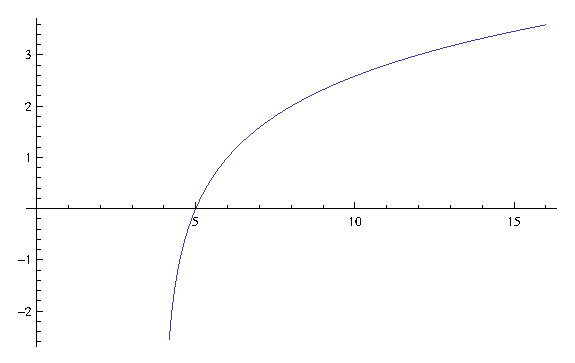
\includegraphics[scale = 0.9]{problem49.eps}
        \caption{Problem 49: $f(x) = \log_2(x - 4)$}
      \end{figure}

    \item[50]
      \begin{tabular}[H]{lll}
        \toprule
        domain    & $(0, \infty)$ \\
        range     & $(-\infty, \infty)$ \\
        asymptote & $x = 0$ \\
        \bottomrule
      \end{tabular}

      \begin{figure}[H]
        \centering
        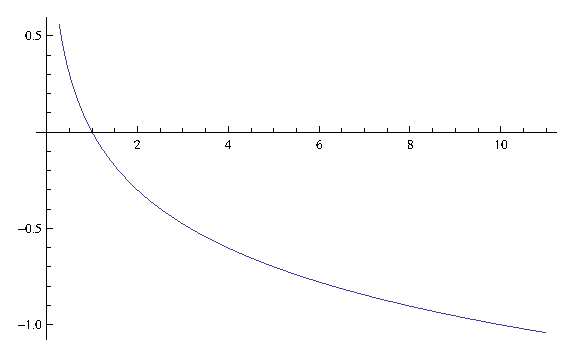
\includegraphics[scale = 0.9]{problem50.eps}
        \caption{Problem 50: $f(x) = -\log_{10} x$}
      \end{figure}

    \item[51]
      \begin{tabular}[H]{lll}
        \toprule
        domain    & $(-\infty, 0)$ \\
        range     & $(-\infty, \infty)$ \\
        asymptote & $x = 0$ \\
        \bottomrule
      \end{tabular}

      \begin{figure}[H]
        \centering
        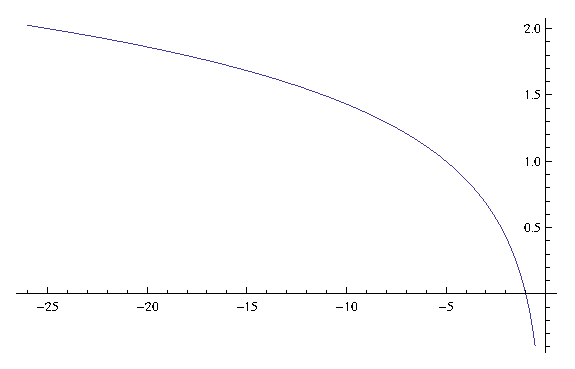
\includegraphics[scale = 0.9]{problem51.eps}
        \caption{Problem 51: $f(x) = \log_{5} (-x)$}
      \end{figure}

    \item[52]
      \begin{tabular}[H]{lll}
        \toprule
        domain    & $(-2, \infty)$ \\
        range     & $(-\infty, \infty)$ \\
        asymptote & $x = -2$ \\
        \bottomrule
      \end{tabular}

      \begin{figure}[H]
        \centering
        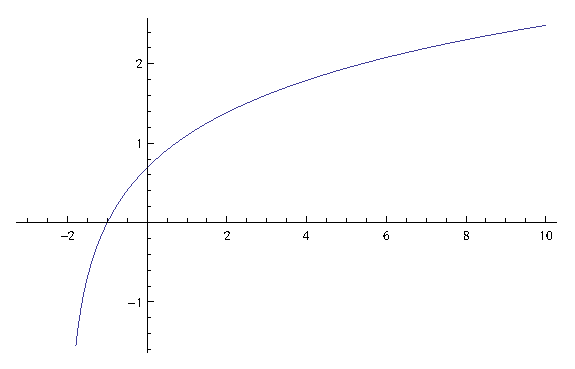
\includegraphics[scale = 0.9]{problem52.eps}
        \caption{Problem 52: $f(x) = \ln(x + 2)$}
      \end{figure}

    \item[53]
      \begin{tabular}[H]{lll}
        \toprule
        domain    & $(0, \infty)$ \\
        range     & $(-\infty, \infty)$ \\
        asymptote & $x = 0$ \\
        \bottomrule
      \end{tabular}

      \begin{figure}[H]
        \centering
        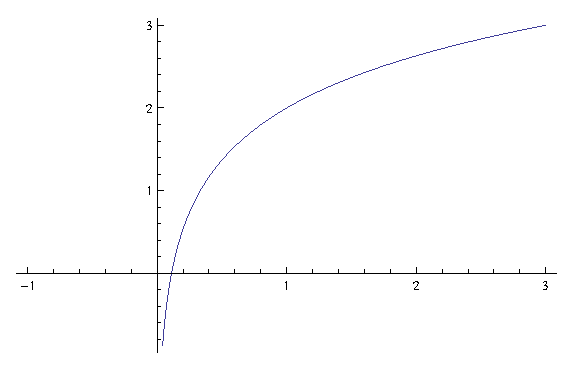
\includegraphics[scale = 0.9]{problem53.eps}
        \caption{Problem 53: $f(x) = 2 + \log_3 x$}
      \end{figure}

    \item[54]
      \begin{tabular}[H]{lll}
        \toprule
        domain    & $(1, \infty)$ \\
        range     & $(-\infty, \infty)$ \\
        asymptote & $x = 1$ \\
        \bottomrule
      \end{tabular}

      \begin{figure}[H]
        \centering
        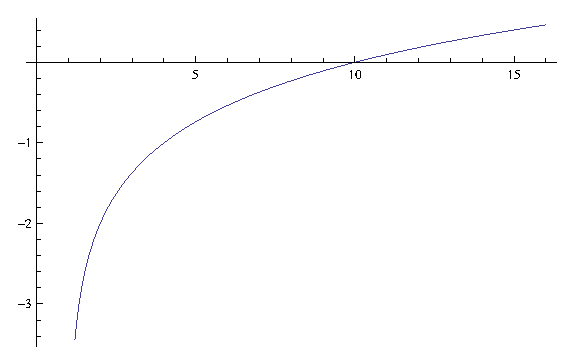
\includegraphics[scale = 0.9]{problem54.eps}
        \caption{Problem 54: $f(x) = \log_3(x - 1) - 2$}
      \end{figure}

    % \item[57]
    %   \begin{tabular}[H]{lll}
    %     \toprule
    %     domain    & $(0, \infty)$ \\
    %     range     & $[0, \infty)$ \\
    %     asymptote & $x = 0$ \\
    %     \bottomrule
    %   \end{tabular}

    %   \begin{figure}[H]
    %     \centering
    %     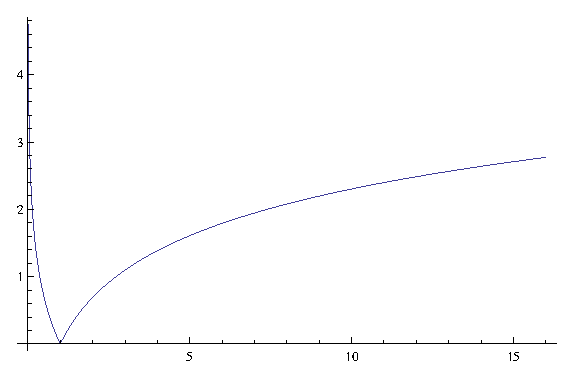
\includegraphics[scale = 0.9]{problem57.eps}
    %     \caption{Problem 57: $f(x) = | \ln x |$}
    %   \end{figure}

    \item[58]
      \begin{tabular}[H]{lll}
        \toprule
        domain    & $(-\infty, 0) \cup (0, \infty)$ \\
        range     & $[-\infty, \infty)$ \\
        asymptote & $x = 0$ \\
        \bottomrule
      \end{tabular}

      \begin{figure}[H]
        \centering
        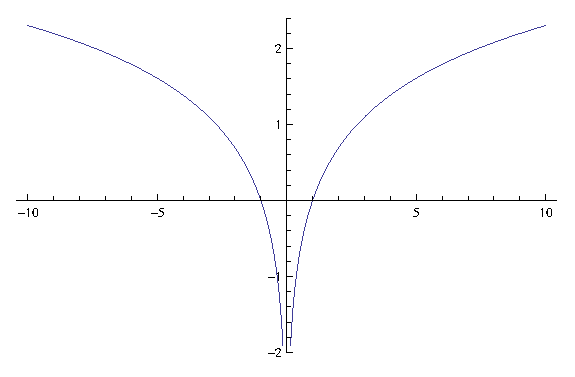
\includegraphics[scale = 0.9]{problem58.eps}
        \caption{Problem 58: $f(x) = \ln |x|$}
      \end{figure}

    \item[59]
      \begin{align*}
        x + 3 & > 0 \\
        x     & > -3 \\
      \end{align*}

      \fbox{$(-3, \infty)$} 

    \item[60]
      \begin{align*}
        8 - 2x & > 0 \\
        2x     & < 8 \\
        x      & < 4 \\
      \end{align*}

      \fbox{$(-\infty, 4)$} 

    \pagebreak

    \item[61]
      \begin{align*}
        x^2 - 1 & > 0 \\
      \end{align*}

      \fbox{$(-\infty, -1) \cup (1, \infty)$} 

    \item[62]
      \begin{align*}
        x - x^2  & > 0 \\
        x(1 - x) & > 0 \\
      \end{align*}

      \fbox{$(0, 1)$} 

    \item[63]
      \begin{align*}
        2 - x & > 0 \\
        x     & < 2 \\
      \end{align*}

      \fbox{$(0, 2)$} 

    \item[64]
      \begin{align*}
        x-2 & >0 \\
        x   & >2 \\
        \\
        10 - x & > 0 \\
        x      & < 10 \\
      \end{align*}

      \fbox{$(2, 10)$} 

    \item[78]
      \begin{align*}
        C &= -2500 \ln \left( \frac{0.7 I_0}{I_0} \right) \\
          &= -2500 \ln 0.7 \\
          &\approx \boxed{\unit[892]{moles/liter}} \\
      \end{align*}

    \item[79]
      \begin{align*}
        A &= -8267 \ln \left( \frac{0.73 D_0}{D_0} \right) \\
          &= -8267  \ln 0.73 \\
          &\approx \boxed{\unit[2602]{years}} \\
      \end{align*}

    \item[80]
      \begin{align*}
        t &= 3 \frac{\log(1,000,000 / 50)}{\log 2} \\
          &\approx \boxed{\unit[43]{hours}} \\
      \end{align*}

    \item[81]
      \begin{tabular}[H]{lr}
        \toprule
        rate & time \\
        \midrule
        6\% & \unit[11.5]{years} \\
        7\% & \unit[9.9]{years} \\
        8\% & \unit[8.7]{years} \\
        \bottomrule
      \end{tabular}
    \end{description}

  \else
    \vspace{2 cm}
    \begin{quote}
      \begin{em}
        Our heart glows, and secret unrest gnaws at the root of our being.
      \end{em}
    \end{quote}

    \hspace{1 cm} --Carl Jung
  \fi

\end{document}

